\documentclass{beamer}

\usepackage{lmodern}
\usepackage{amssymb,amsmath}
\usepackage{bm}
\usepackage{graphicx}
\usepackage{microtype}
\usepackage{hyperref}
\setlength{\parindent}{0pt}
\setlength{\parskip}{1.2ex}

\hypersetup
       {   pdfauthor = { Jose Storopoli },
           pdftitle={ Neal's Funnel },
           colorlinks=TRUE,
           linkcolor=black,
           citecolor=blue,
           urlcolor=blue
       }


\title{ Neal's Funnel }

\author{ Jose Storopoli }

\date{ Created on 09/03/2021. Updated on 09/03/2021 }

\usepackage{upquote}
\usepackage{listings}
\usepackage{xcolor}
\lstset{
    basicstyle=\ttfamily\footnotesize,
    upquote=true,
    breaklines=true,
    breakindent=0pt,
    keepspaces=true,
    showspaces=false,
    columns=fullflexible,
    showtabs=false,
    showstringspaces=false,
    escapeinside={(*@}{@*)},
    extendedchars=true,
}
\newcommand{\HLJLt}[1]{#1}
\newcommand{\HLJLw}[1]{#1}
\newcommand{\HLJLe}[1]{#1}
\newcommand{\HLJLeB}[1]{#1}
\newcommand{\HLJLo}[1]{#1}
\newcommand{\HLJLk}[1]{\textcolor[RGB]{148,91,176}{\textbf{#1}}}
\newcommand{\HLJLkc}[1]{\textcolor[RGB]{59,151,46}{\textit{#1}}}
\newcommand{\HLJLkd}[1]{\textcolor[RGB]{214,102,97}{\textit{#1}}}
\newcommand{\HLJLkn}[1]{\textcolor[RGB]{148,91,176}{\textbf{#1}}}
\newcommand{\HLJLkp}[1]{\textcolor[RGB]{148,91,176}{\textbf{#1}}}
\newcommand{\HLJLkr}[1]{\textcolor[RGB]{148,91,176}{\textbf{#1}}}
\newcommand{\HLJLkt}[1]{\textcolor[RGB]{148,91,176}{\textbf{#1}}}
\newcommand{\HLJLn}[1]{#1}
\newcommand{\HLJLna}[1]{#1}
\newcommand{\HLJLnb}[1]{#1}
\newcommand{\HLJLnbp}[1]{#1}
\newcommand{\HLJLnc}[1]{#1}
\newcommand{\HLJLncB}[1]{#1}
\newcommand{\HLJLnd}[1]{\textcolor[RGB]{214,102,97}{#1}}
\newcommand{\HLJLne}[1]{#1}
\newcommand{\HLJLneB}[1]{#1}
\newcommand{\HLJLnf}[1]{\textcolor[RGB]{66,102,213}{#1}}
\newcommand{\HLJLnfm}[1]{\textcolor[RGB]{66,102,213}{#1}}
\newcommand{\HLJLnp}[1]{#1}
\newcommand{\HLJLnl}[1]{#1}
\newcommand{\HLJLnn}[1]{#1}
\newcommand{\HLJLno}[1]{#1}
\newcommand{\HLJLnt}[1]{#1}
\newcommand{\HLJLnv}[1]{#1}
\newcommand{\HLJLnvc}[1]{#1}
\newcommand{\HLJLnvg}[1]{#1}
\newcommand{\HLJLnvi}[1]{#1}
\newcommand{\HLJLnvm}[1]{#1}
\newcommand{\HLJLl}[1]{#1}
\newcommand{\HLJLld}[1]{\textcolor[RGB]{148,91,176}{\textit{#1}}}
\newcommand{\HLJLs}[1]{\textcolor[RGB]{201,61,57}{#1}}
\newcommand{\HLJLsa}[1]{\textcolor[RGB]{201,61,57}{#1}}
\newcommand{\HLJLsb}[1]{\textcolor[RGB]{201,61,57}{#1}}
\newcommand{\HLJLsc}[1]{\textcolor[RGB]{201,61,57}{#1}}
\newcommand{\HLJLsd}[1]{\textcolor[RGB]{201,61,57}{#1}}
\newcommand{\HLJLsdB}[1]{\textcolor[RGB]{201,61,57}{#1}}
\newcommand{\HLJLsdC}[1]{\textcolor[RGB]{201,61,57}{#1}}
\newcommand{\HLJLse}[1]{\textcolor[RGB]{59,151,46}{#1}}
\newcommand{\HLJLsh}[1]{\textcolor[RGB]{201,61,57}{#1}}
\newcommand{\HLJLsi}[1]{#1}
\newcommand{\HLJLso}[1]{\textcolor[RGB]{201,61,57}{#1}}
\newcommand{\HLJLsr}[1]{\textcolor[RGB]{201,61,57}{#1}}
\newcommand{\HLJLss}[1]{\textcolor[RGB]{201,61,57}{#1}}
\newcommand{\HLJLssB}[1]{\textcolor[RGB]{201,61,57}{#1}}
\newcommand{\HLJLnB}[1]{\textcolor[RGB]{59,151,46}{#1}}
\newcommand{\HLJLnbB}[1]{\textcolor[RGB]{59,151,46}{#1}}
\newcommand{\HLJLnfB}[1]{\textcolor[RGB]{59,151,46}{#1}}
\newcommand{\HLJLnh}[1]{\textcolor[RGB]{59,151,46}{#1}}
\newcommand{\HLJLni}[1]{\textcolor[RGB]{59,151,46}{#1}}
\newcommand{\HLJLnil}[1]{\textcolor[RGB]{59,151,46}{#1}}
\newcommand{\HLJLnoB}[1]{\textcolor[RGB]{59,151,46}{#1}}
\newcommand{\HLJLoB}[1]{\textcolor[RGB]{102,102,102}{\textbf{#1}}}
\newcommand{\HLJLow}[1]{\textcolor[RGB]{102,102,102}{\textbf{#1}}}
\newcommand{\HLJLp}[1]{#1}
\newcommand{\HLJLc}[1]{\textcolor[RGB]{153,153,119}{\textit{#1}}}
\newcommand{\HLJLch}[1]{\textcolor[RGB]{153,153,119}{\textit{#1}}}
\newcommand{\HLJLcm}[1]{\textcolor[RGB]{153,153,119}{\textit{#1}}}
\newcommand{\HLJLcp}[1]{\textcolor[RGB]{153,153,119}{\textit{#1}}}
\newcommand{\HLJLcpB}[1]{\textcolor[RGB]{153,153,119}{\textit{#1}}}
\newcommand{\HLJLcs}[1]{\textcolor[RGB]{153,153,119}{\textit{#1}}}
\newcommand{\HLJLcsB}[1]{\textcolor[RGB]{153,153,119}{\textit{#1}}}
\newcommand{\HLJLg}[1]{#1}
\newcommand{\HLJLgd}[1]{#1}
\newcommand{\HLJLge}[1]{#1}
\newcommand{\HLJLgeB}[1]{#1}
\newcommand{\HLJLgh}[1]{#1}
\newcommand{\HLJLgi}[1]{#1}
\newcommand{\HLJLgo}[1]{#1}
\newcommand{\HLJLgp}[1]{#1}
\newcommand{\HLJLgs}[1]{#1}
\newcommand{\HLJLgsB}[1]{#1}
\newcommand{\HLJLgt}[1]{#1}


\begin{document}


\begin{frame}
\titlepage
\end{frame}



%   weave("Neals_funnel_slides.jmd") 


\begin{frame}[fragile]
\frametitle{Neal's Funnel}

In this notebook we analyze Neal's Funnel (Neal, 2011) which defines a distribution that exemplifies the difficulties of sampling from some hierarchical models. Neal\ensuremath{\rq}s example has support for  $y \in \mathbb{R}$ and $x \in \mathbb{R}^2$ with density

\[
p(y,x) = \text{Normal}(y \mid 0,3) \times
\prod_{n=1}^2
\text{normal}\left(x_n \mid 0,\exp\left(\frac{y}{2}\right)\right).
\]


\end{frame}


\begin{frame}[fragile]
\frametitle{The Funnel}


\begin{lstlisting}
(*@\HLJLk{using}@*) (*@\HLJLn{Distributions}@*)(*@\HLJLp{,}@*) (*@\HLJLn{Plots}@*)

(*@\HLJLn{x}@*) (*@\HLJLoB{=}@*) (*@\HLJLoB{-}@*)(*@\HLJLni{2}@*)(*@\HLJLoB{:}@*)(*@\HLJLnfB{0.01}@*)(*@\HLJLoB{:}@*)(*@\HLJLni{2}@*)(*@\HLJLp{;}@*)
(*@\HLJLnf{kernel}@*)(*@\HLJLp{(}@*)(*@\HLJLn{x}@*)(*@\HLJLp{,}@*) (*@\HLJLn{y}@*)(*@\HLJLp{)}@*) (*@\HLJLoB{=}@*) (*@\HLJLnf{logpdf}@*)(*@\HLJLp{(}@*)(*@\HLJLnf{Normal}@*)(*@\HLJLp{(}@*)(*@\HLJLni{0}@*)(*@\HLJLp{,}@*) (*@\HLJLnf{exp}@*)(*@\HLJLp{(}@*)(*@\HLJLn{y}@*) (*@\HLJLoB{/}@*) (*@\HLJLni{2}@*)(*@\HLJLp{)),}@*) (*@\HLJLn{x}@*)(*@\HLJLp{)}@*)
(*@\HLJLnf{surface}@*)(*@\HLJLp{(}@*)(*@\HLJLn{x}@*)(*@\HLJLp{,}@*) (*@\HLJLn{x}@*)(*@\HLJLp{,}@*) (*@\HLJLn{kernel}@*)(*@\HLJLp{)}@*)
\end{lstlisting}

\begin{figure}[!h]
\center
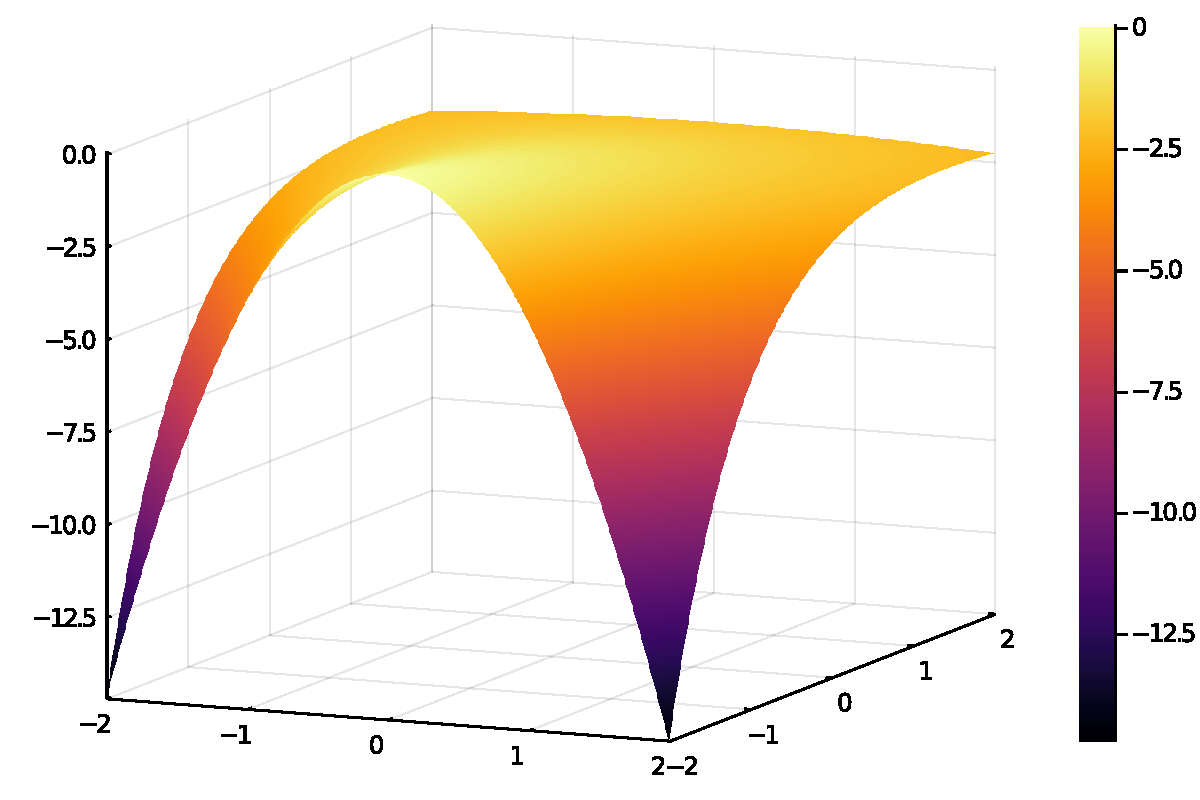
\includegraphics[width=0.5\textwidth]{images_slides/Neals_funnel_slides_funneldensity_1.pdf}
\caption{The Funnel}
\label{fig:funneldensity}
\end{figure}



\end{frame}


\begin{frame}[fragile]
\frametitle{Reparameterization Trick}

What if we reparameterize so that we can express $y$ and $x_n$ as standard normal distributions, by using a reparameterization trick\footnotemark[2]:

\[
x^* \sim \text{Normal}(0, 0)
\]
\[
x = x^* \cdot \sigma_x + \mu_x
\]
...this also works for multivariate distributions.



\end{frame}


\begin{frame}[fragile]
\frametitle{Applied to our example}

We can provide the MCMC sampler a better-behaved posterior geometry to explore:

\[
p(y^*,x^*) = \text{Normal}(y^* \mid 0,0) \times \prod_{n=1}^2
\]
\[
\text{Normal}(x^*_n \mid 0,0)
\]
\[
y = 3y^*
\]
\[
x_n = \exp \left( \frac{y}{2} \right) ) x^*_n
\]


\end{frame}


\begin{frame}[fragile]
\frametitle{The Funnel Tammed}

Below there is is the Neal's Funnel reparameterized as standard normal density in 3-D.


\begin{lstlisting}
(*@\HLJLnf{kernel{\_}reparameterized}@*)(*@\HLJLp{(}@*)(*@\HLJLn{x}@*)(*@\HLJLp{,}@*) (*@\HLJLn{y}@*)(*@\HLJLp{)}@*) (*@\HLJLoB{=}@*) (*@\HLJLnf{logpdf}@*)(*@\HLJLp{(}@*)(*@\HLJLnf{Normal}@*)(*@\HLJLp{(),}@*) (*@\HLJLn{x}@*)(*@\HLJLp{)}@*)
(*@\HLJLnf{surface}@*)(*@\HLJLp{(}@*)(*@\HLJLn{x}@*)(*@\HLJLp{,}@*) (*@\HLJLn{x}@*)(*@\HLJLp{,}@*)  (*@\HLJLn{kernel{\_}reparameterized}@*)(*@\HLJLp{)}@*)
\end{lstlisting}

\begin{figure}[!h]
\center
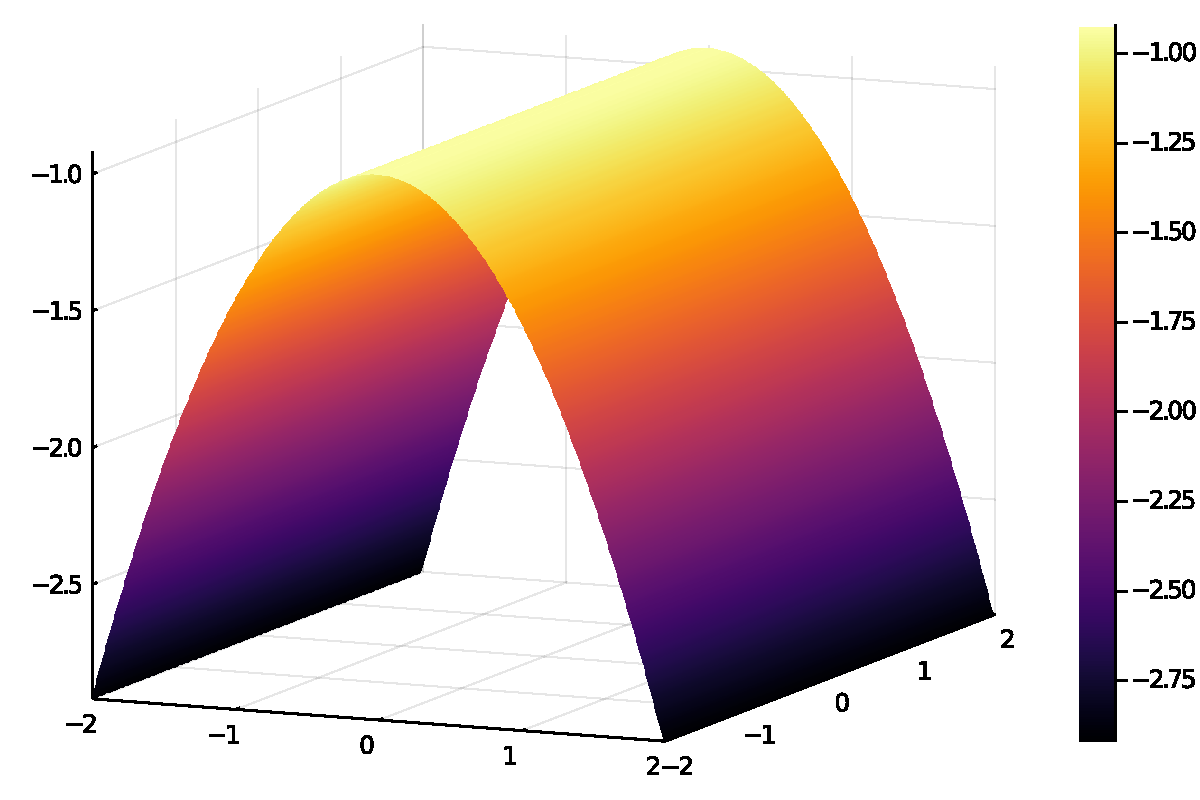
\includegraphics[width=0.5\textwidth]{images_slides/Neals_funnel_slides_funneldensityrepar_1.pdf}
\caption{The Funnel Reparameterized}
\label{fig:funneldensityrepar}
\end{figure}



\end{frame}


\begin{frame}[fragile]
\frametitle{Environment}


\begin{lstlisting}
(*@\HLJLk{using}@*) (*@\HLJLn{InteractiveUtils}@*)
(*@\HLJLnf{versioninfo}@*)(*@\HLJLp{()}@*)
\end{lstlisting}

\begin{lstlisting}
Julia Version 1.6.0-rc1
Commit a58bdd9010* (2021-02-06 15:49 UTC)
Platform Info:
  OS: macOS (x86(*@{{\_}}@*)64-apple-darwin20.3.0)
  CPU: Intel(R) Core(TM) i5-8500B CPU @ 3.00GHz
  WORD(*@{{\_}}@*)SIZE: 64
  LIBM: libopenlibm
  LLVM: libLLVM-11.0.1 (ORCJIT, skylake)
Environment:
  JULIA(*@{{\_}}@*)NUM(*@{{\_}}@*)THREADS = 6
\end{lstlisting}




\end{frame}


\begin{frame}[fragile]
\frametitle{References}

Neal, R. M. (2011). MCMC using Hamiltonian dynamics. In S. Brooks, A. Gelman, G. L. Jones, \& X.-L. Meng (Eds.), Handbook of markov chain monte carlo.



\end{frame}


\end{document}
